\documentclass[handout]{beamer}
% L'option handout permet de supprimer la barre de navigation

\usepackage[T1]{fontenc}
\usepackage[utf8]{inputenc}
\usepackage[french]{babel}
% Pour utiliser le signe €
\usepackage{eurosym}
% Pour pouvoir insérer des images
\usepackage{graphicx}
\usepackage{wrapfig}
% Gestion des couleurs
\usepackage{color}
\definecolor{QTPurple}{RGB}{61, 68, 160}
% Coloration syntaxique
\usepackage{listings}
\lstset{ 
	language=PHP,
	numbers=left,
	showstringspaces=false, 
	tabsize=4,
	breaklines=true,
	extendedchars=true,
	literate={é}{{\'e}}1 {à}{{\`a}}1 {è}{{\`e}}1 {ç}{{\c c}}1
}

% Un joli thème flat
\usetheme{Rochester}

% Personnalisation du thème
\usecolortheme[named=QTPurple]{structure}
\setbeamertemplate{blocks}[shadow=false]

% Générer une page de titre à chaque début de section
\AtBeginSection[]
{
	\begin{frame}[plain]
	\frametitle{Sommaire}
	\tableofcontents[currentsection, hideothersubsections]
	\end{frame} 
}

% Affichage du logo Quantic Télécom en bas de chaque slide
\logo{
\includegraphics[height=10mm]{images/logo.png}}

% ------------------------------------ %
% -- METADONNÉES DU DOCUMENT --------- %
\title[Quantic]{
	Quantic Télécom\\
	Point sur la situation actuelle et projets en cours
}
\author{
	Antoine Augusti, 
	Étienne Batise
}
\date{Février 2014}

\titlegraphic{
\includegraphics[height=.3\textheight]{images/logo.png}}

% Début du document
\begin{document}
	
	% Génération de la page de titre
	\begin{frame}[plain]
		\titlepage
	\end{frame}

	% Génération du sommaire
	\begin{frame}[plain]
		\frametitle{Sommaire}
		\tableofcontents
	\end{frame}


	% ///////////////////////////////////////////////////////// %
	% /// Quantic Télécom actuellement /////////////////////// %
	\section{Quantic Télécom actuellement}

	\subsection{Public couvert aujourd'hui}
		\begin{frame}
		\frametitle{Public couvert aujourd'hui}
		\begin{tabular}{l l}
			\begin{minipage}{0.2\textwidth}
				\begin{center}
					
\includegraphics[width=0.9\textwidth]{images/residence.png}
				\end{center}
			\end{minipage}

			\begin{minipage}{0.8\textwidth}
				\begin{itemize}
					\item couverture de toutes les résidences de l'INSA de Rouen
					\item présent dans 2 résidences du CROUS : Malibran et Emma Bovary
					\item 650 adhérents cette année
					\item 7 personnes impliquées dans le projet
				\end{itemize}
			\end{minipage}
			
		\end{tabular}
		\end{frame}

	\subsection{Le réseau actuel}
		\begin{frame}
		\frametitle{Le réseau actuel}
		\vspace{-20px}
		\begin{center}
			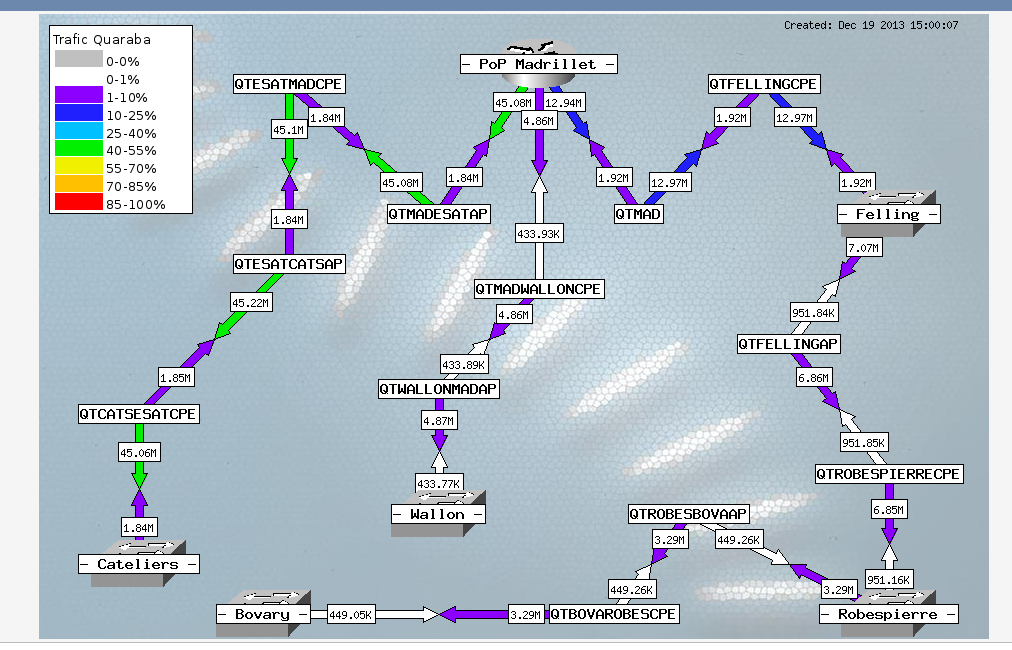
\includegraphics[width=0.9\textwidth]{images/cacti.png}
		\end{center}
		
		\end{frame}

	\subsection{Un exemple d'antennes}
		\begin{frame}
		\frametitle{Un exemple d'antennes}
		\begin{tabular}{l l}
			\begin{minipage}{0.4\textwidth}
				\begin{center}
					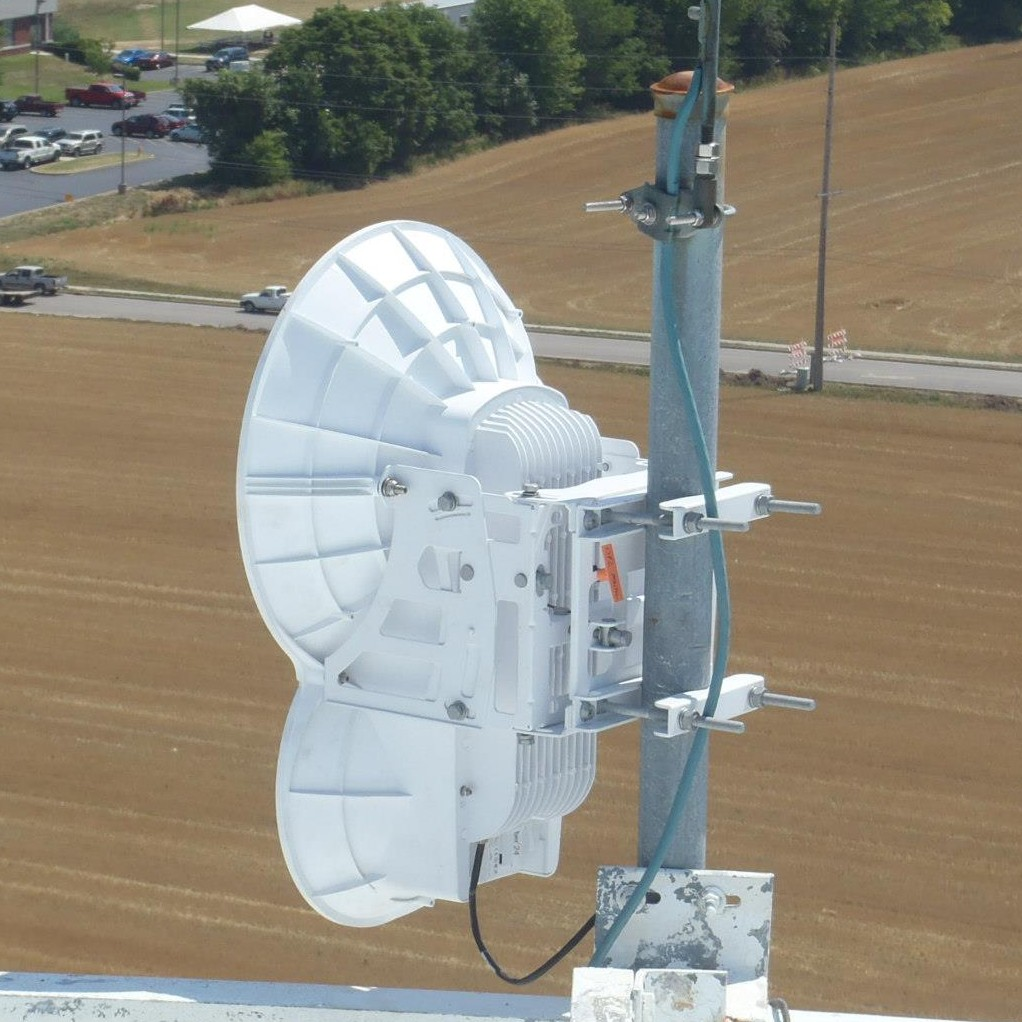
\includegraphics[width=0.9\textwidth]{images/airFiber.jpg}
				\end{center}
			\end{minipage}

			\begin{minipage}{0.6\textwidth}
				\begin{itemize}
					\item antennes point à point, unidirectionnelles
					\item puissance d'émission inférieure à un téléphone portable
					\item longue portée : jusqu'à 15km sans obstacles
					\item prix \textit{relativement} correct
				\end{itemize}
			\end{minipage}
			
		\end{tabular}
		\end{frame}
	% ///////////////////////////////////////////////////////// %


	% ///////////////////////////////////////////////////// %
	% /// Dysfonctionnements en cours ///////////////////// %
	\section{Dysfonctionnements en cours}

	\subsection{Couverture réseau dans les résidences}
		\begin{frame}
		\frametitle{Couverture réseau dans les résidences}

		\begin{tabular}{l l}
			\begin{minipage}{0.2\textwidth}
				\begin{center}
					
\includegraphics[width=0.9\textwidth]{images/internet.png}
				\end{center}
			\end{minipage}

			\begin{minipage}{0.8\textwidth}
				\begin{itemize}
					\item instabilité du réseau en début d'année scolaire
					\begin{itemize}
						\item problème de capacité de notre réseau
						\item attaques
						\item coupures électriques
					\end{itemize}
					\item problème de couverture Wi-Fi à Felling et aux Cateliers
				\end{itemize}
			\end{minipage}
			
		\end{tabular}
		\end{frame}

	\subsection{Manque de communication}
		\begin{frame}
		\frametitle{Manque de communication}

		\begin{tabular}{l l}
			\begin{minipage}{0.2\textwidth}
				\begin{center}
					
\includegraphics[width=0.9\textwidth]{images/communication.png}
				\end{center}
			\end{minipage}

			\begin{minipage}{0.8\textwidth}
				\begin{itemize}
					\item manque de communication envers nos adhérents
					\item impression de non-réaction en cas de problème
					\item difficultés pour nos adhérents de connaître le rôle que nous jouons
					\item mauvaise remontée des problèmes par nos adhérents
				\end{itemize}
			\end{minipage}
			
		\end{tabular}
		\end{frame}

	% //////////////////////////////////////////////////// %
	% /// Projets en cours ////////////////////////////// %
	\section{Projets en cours}

	\subsection{Projet Quaraba}
		\begin{frame}
		\frametitle{Projet Quaraba}

		\begin{tabular}{l l}
			\begin{minipage}{0.2\textwidth}
				\begin{center}
					
\includegraphics[width=0.9\textwidth]{images/antennes.png}
				\end{center}
			\end{minipage}

			\begin{minipage}{0.8\textwidth}
				\begin{itemize}
					\item dorsales de notre réseau assurées par des liaisons hertziennes
					\item projet Quaraba : \textit{Quantic radioelectrical backbone}
					\item utilisation d'antennes de nouvelle génération
					\item besoin de points hauts pour relier les résidences à notre backbone
					\item besoin d'un relai sur la Côte Sainte-Catherine
				\end{itemize}
			\end{minipage}
			
		\end{tabular}
		\end{frame}

	\subsection{Futur backbone}
		\begin{frame}
		\frametitle{Futur backbone}
		\vspace{-5px}
		\begin{center}
			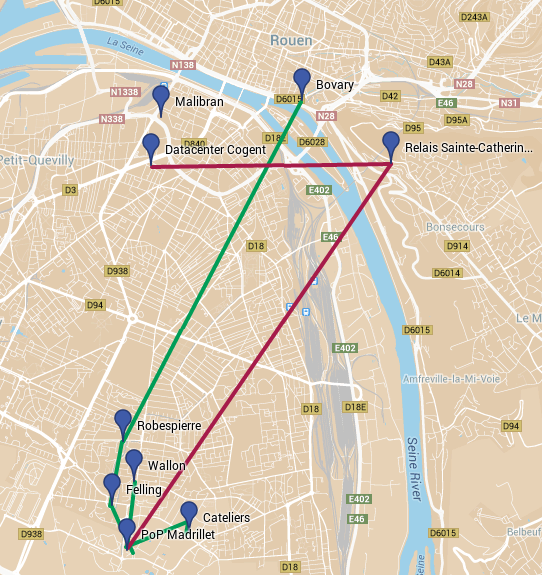
\includegraphics[width=0.70\textwidth]{images/futurReseau.png}
		\end{center}
		
		\end{frame}

	% //////////////////////////////////////////////////// %
	% /// Comment vous investir ////////////////////////// %
	\section{Comment vous investir}
	\begin{frame}
	\frametitle{Comment s'investir}

	\begin{tabular}{l l}
		\begin{minipage}{0.2\textwidth}
			\begin{center}
				
\includegraphics[width=0.9\textwidth]{images/equipe.png}
			\end{center}
		\end{minipage}

		\begin{minipage}{0.8\textwidth}
			\begin{itemize}
				\item remonter les problèmes que vous rencontrez par notre système de tickets
				\item nous contacter quand vous souhaitez avoir des informations ou que vous avez des questions
				\item pourquoi pas rejoindre notre équipe ?
				\begin{itemize}
					\item découverte de la dimension physique de l'Internet
					\item plus \textbf{énorme} pour votre CV
					\item apprentissage technique bien plus poussé que les cours
					\item mise en place d'un réseau professionnel
				\end{itemize}
			\end{itemize}
		\end{minipage}
		
	\end{tabular}
	\end{frame}


% Fin du document
\end{document}
